% Created by tikzDevice version 0.12.3.1 on 2021-11-16 08:52:23
% !TEX encoding = UTF-8 Unicode
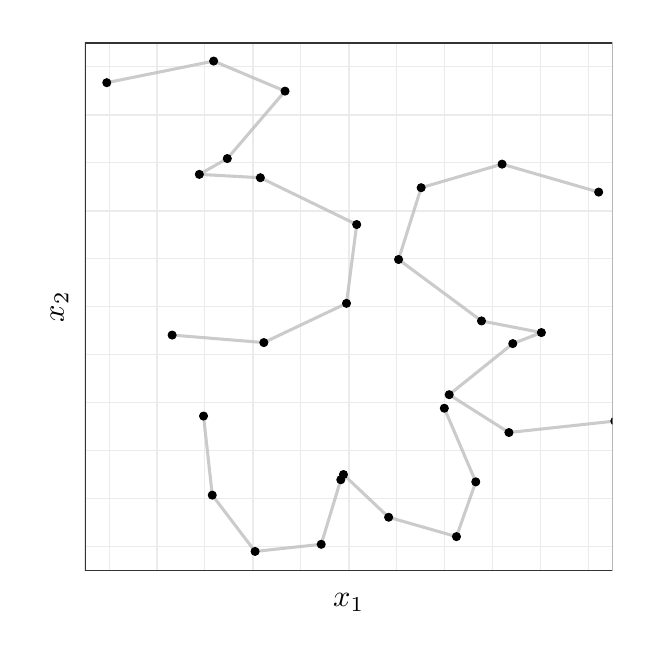
\begin{tikzpicture}[x=1pt,y=1pt]
\definecolor{fillColor}{RGB}{255,255,255}
\path[use as bounding box,fill=fillColor,fill opacity=0.00] (0,0) rectangle (216.81,216.81);
\begin{scope}
\path[clip] (  0.00,  0.00) rectangle (216.81,216.81);
\definecolor{drawColor}{RGB}{255,255,255}
\definecolor{fillColor}{RGB}{255,255,255}

\path[draw=drawColor,line width= 0.6pt,line join=round,line cap=round,fill=fillColor] (  0.00,  0.00) rectangle (216.81,216.81);
\end{scope}
\begin{scope}
\path[clip] ( 20.71, 20.71) rectangle (211.31,211.31);
\definecolor{fillColor}{RGB}{255,255,255}

\path[fill=fillColor] ( 20.71, 20.71) rectangle (211.31,211.31);
\definecolor{drawColor}{gray}{0.92}

\path[draw=drawColor,line width= 0.3pt,line join=round] ( 20.71, 29.38) --
	(211.31, 29.38);

\path[draw=drawColor,line width= 0.3pt,line join=round] ( 20.71, 64.03) --
	(211.31, 64.03);

\path[draw=drawColor,line width= 0.3pt,line join=round] ( 20.71, 98.69) --
	(211.31, 98.69);

\path[draw=drawColor,line width= 0.3pt,line join=round] ( 20.71,133.34) --
	(211.31,133.34);

\path[draw=drawColor,line width= 0.3pt,line join=round] ( 20.71,167.99) --
	(211.31,167.99);

\path[draw=drawColor,line width= 0.3pt,line join=round] ( 20.71,202.65) --
	(211.31,202.65);

\path[draw=drawColor,line width= 0.3pt,line join=round] ( 29.38, 20.71) --
	( 29.38,211.31);

\path[draw=drawColor,line width= 0.3pt,line join=round] ( 64.03, 20.71) --
	( 64.03,211.31);

\path[draw=drawColor,line width= 0.3pt,line join=round] ( 98.69, 20.71) --
	( 98.69,211.31);

\path[draw=drawColor,line width= 0.3pt,line join=round] (133.34, 20.71) --
	(133.34,211.31);

\path[draw=drawColor,line width= 0.3pt,line join=round] (167.99, 20.71) --
	(167.99,211.31);

\path[draw=drawColor,line width= 0.3pt,line join=round] (202.65, 20.71) --
	(202.65,211.31);

\path[draw=drawColor,line width= 0.6pt,line join=round] ( 20.71, 46.70) --
	(211.31, 46.70);

\path[draw=drawColor,line width= 0.6pt,line join=round] ( 20.71, 81.36) --
	(211.31, 81.36);

\path[draw=drawColor,line width= 0.6pt,line join=round] ( 20.71,116.01) --
	(211.31,116.01);

\path[draw=drawColor,line width= 0.6pt,line join=round] ( 20.71,150.67) --
	(211.31,150.67);

\path[draw=drawColor,line width= 0.6pt,line join=round] ( 20.71,185.32) --
	(211.31,185.32);

\path[draw=drawColor,line width= 0.6pt,line join=round] ( 46.70, 20.71) --
	( 46.70,211.31);

\path[draw=drawColor,line width= 0.6pt,line join=round] ( 81.36, 20.71) --
	( 81.36,211.31);

\path[draw=drawColor,line width= 0.6pt,line join=round] (116.01, 20.71) --
	(116.01,211.31);

\path[draw=drawColor,line width= 0.6pt,line join=round] (150.67, 20.71) --
	(150.67,211.31);

\path[draw=drawColor,line width= 0.6pt,line join=round] (185.32, 20.71) --
	(185.32,211.31);
\definecolor{drawColor}{RGB}{190,190,190}

\path[draw=drawColor,draw opacity=0.80,line width= 1.1pt,line join=round] ( 63.55, 76.47) --
	( 66.70, 47.89) --
	( 82.17, 27.55) --
	(106.07, 30.13) --
	(113.14, 53.46) --
	(114.11, 55.34) --
	(130.43, 39.90) --
	(154.94, 32.90) --
	(161.92, 52.69) --
	(150.55, 79.29);

\path[draw=drawColor,draw opacity=0.80,line width= 1.1pt,line join=round] (206.33,157.39) --
	(171.42,167.50) --
	(142.18,158.98) --
	(134.02,133.04) --
	(163.99,110.84) --
	(185.63,106.63) --
	(175.29,102.65) --
	(152.31, 84.19) --
	(173.90, 70.52) --
	(212.18, 74.65);

\path[draw=drawColor,draw opacity=0.80,line width= 1.1pt,line join=round] ( 52.20,105.73) --
	( 85.34,103.02) --
	(115.20,117.19) --
	(118.89,145.67) --
	( 84.08,162.59) --
	( 62.03,163.80) --
	( 72.13,169.51) --
	( 93.00,193.88) --
	( 67.20,204.74) --
	( 28.58,196.93);
\definecolor{drawColor}{RGB}{0,0,0}
\definecolor{fillColor}{RGB}{0,0,0}

\path[draw=drawColor,line width= 0.4pt,line join=round,line cap=round,fill=fillColor] ( 63.55, 76.47) circle (  1.43);

\path[draw=drawColor,line width= 0.4pt,line join=round,line cap=round,fill=fillColor] ( 66.70, 47.89) circle (  1.43);

\path[draw=drawColor,line width= 0.4pt,line join=round,line cap=round,fill=fillColor] ( 82.17, 27.55) circle (  1.43);

\path[draw=drawColor,line width= 0.4pt,line join=round,line cap=round,fill=fillColor] (106.07, 30.13) circle (  1.43);

\path[draw=drawColor,line width= 0.4pt,line join=round,line cap=round,fill=fillColor] (113.14, 53.46) circle (  1.43);

\path[draw=drawColor,line width= 0.4pt,line join=round,line cap=round,fill=fillColor] (114.11, 55.34) circle (  1.43);

\path[draw=drawColor,line width= 0.4pt,line join=round,line cap=round,fill=fillColor] (130.43, 39.90) circle (  1.43);

\path[draw=drawColor,line width= 0.4pt,line join=round,line cap=round,fill=fillColor] (154.94, 32.90) circle (  1.43);

\path[draw=drawColor,line width= 0.4pt,line join=round,line cap=round,fill=fillColor] (161.92, 52.69) circle (  1.43);

\path[draw=drawColor,line width= 0.4pt,line join=round,line cap=round,fill=fillColor] (150.55, 79.29) circle (  1.43);

\path[draw=drawColor,line width= 0.4pt,line join=round,line cap=round,fill=fillColor] (206.33,157.39) circle (  1.43);

\path[draw=drawColor,line width= 0.4pt,line join=round,line cap=round,fill=fillColor] (171.42,167.50) circle (  1.43);

\path[draw=drawColor,line width= 0.4pt,line join=round,line cap=round,fill=fillColor] (142.18,158.98) circle (  1.43);

\path[draw=drawColor,line width= 0.4pt,line join=round,line cap=round,fill=fillColor] (134.02,133.04) circle (  1.43);

\path[draw=drawColor,line width= 0.4pt,line join=round,line cap=round,fill=fillColor] (163.99,110.84) circle (  1.43);

\path[draw=drawColor,line width= 0.4pt,line join=round,line cap=round,fill=fillColor] (185.63,106.63) circle (  1.43);

\path[draw=drawColor,line width= 0.4pt,line join=round,line cap=round,fill=fillColor] (175.29,102.65) circle (  1.43);

\path[draw=drawColor,line width= 0.4pt,line join=round,line cap=round,fill=fillColor] (152.31, 84.19) circle (  1.43);

\path[draw=drawColor,line width= 0.4pt,line join=round,line cap=round,fill=fillColor] (173.90, 70.52) circle (  1.43);

\path[draw=drawColor,line width= 0.4pt,line join=round,line cap=round,fill=fillColor] (212.18, 74.65) circle (  1.43);

\path[draw=drawColor,line width= 0.4pt,line join=round,line cap=round,fill=fillColor] ( 52.20,105.73) circle (  1.43);

\path[draw=drawColor,line width= 0.4pt,line join=round,line cap=round,fill=fillColor] ( 85.34,103.02) circle (  1.43);

\path[draw=drawColor,line width= 0.4pt,line join=round,line cap=round,fill=fillColor] (115.20,117.19) circle (  1.43);

\path[draw=drawColor,line width= 0.4pt,line join=round,line cap=round,fill=fillColor] (118.89,145.67) circle (  1.43);

\path[draw=drawColor,line width= 0.4pt,line join=round,line cap=round,fill=fillColor] ( 84.08,162.59) circle (  1.43);

\path[draw=drawColor,line width= 0.4pt,line join=round,line cap=round,fill=fillColor] ( 62.03,163.80) circle (  1.43);

\path[draw=drawColor,line width= 0.4pt,line join=round,line cap=round,fill=fillColor] ( 72.13,169.51) circle (  1.43);

\path[draw=drawColor,line width= 0.4pt,line join=round,line cap=round,fill=fillColor] ( 93.00,193.88) circle (  1.43);

\path[draw=drawColor,line width= 0.4pt,line join=round,line cap=round,fill=fillColor] ( 67.20,204.74) circle (  1.43);

\path[draw=drawColor,line width= 0.4pt,line join=round,line cap=round,fill=fillColor] ( 28.58,196.93) circle (  1.43);
\definecolor{drawColor}{gray}{0.20}

\path[draw=drawColor,line width= 0.6pt,line join=round,line cap=round] ( 20.71, 20.71) rectangle (211.31,211.31);
\end{scope}
\begin{scope}
\path[clip] (  0.00,  0.00) rectangle (216.81,216.81);
\definecolor{drawColor}{RGB}{0,0,0}

\node[text=drawColor,anchor=base,inner sep=0pt, outer sep=0pt, scale=  1.10] at (116.01,  7.64) {$x_1$};
\end{scope}
\begin{scope}
\path[clip] (  0.00,  0.00) rectangle (216.81,216.81);
\definecolor{drawColor}{RGB}{0,0,0}

\node[text=drawColor,rotate= 90.00,anchor=base,inner sep=0pt, outer sep=0pt, scale=  1.10] at ( 13.08,116.01) {$x_2$};
\end{scope}
\end{tikzpicture}
